The perceptron was first introduced in 1958 by F. Rosenblatt \cite{brain_perceptron_nodate}. It is a computational model based on on the brain. A biological neuron receives information through chemical mechanisms and once a threshold is passed, the cumulate charges are released (we say the neuro fires) and the information is transmitted to other neurons. \newline \newline
Mathematically, a perceptron has n inputs ($x_1$, ..., $x_n$) which can be expressed as vector \textbf{$\bar{x}$}, n wheights (\textbf{$\bar{w}$}) and a bias \textbf{b}. The perceptron, when receiving an input vector, performs a weighted sum. If the wheighted sum is above a threshold (controlled by the bias which can lower or raise it), the perceptron is 'activated' and outputs a non-zero value (1). The figure \ref{fig:perceptron} illustrates this. We can write the operation in a vector form:
$$ h(x| w, b) = h(\sum^{n}_{i=1} x_i \cdot w_i + b) = h ( \textbf{$\bar{w}$}^{T} \textbf{$\bar{x}$} + b) $$
where the function h is the activation function of the perceptron which was desribe as a boolean level function. The section \ref{subs:acti} describes other activation function. \newline \newline
In the following section \ref{subs:fcl}, we present the layer of perceptron (fully connected layer).
\begin{figure}
    \centering
    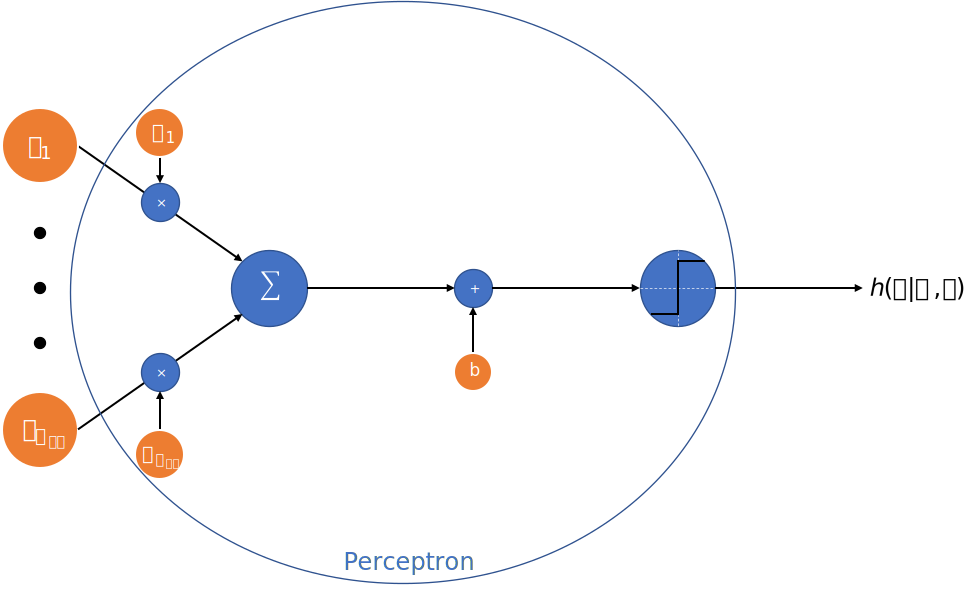
\includegraphics[width=\textwidth]{perceptron.pdf}
    \caption{The Perceptron}
    \label{fig:perceptron}
\end{figure}
